\documentclass[a4paper,12pt]{article}
\usepackage{amsmath}
\usepackage{amsfonts}
\usepackage{geometry}
\geometry{hmargin=2.5cm,vmargin=1.5cm}
\usepackage{amssymb}
\usepackage{graphicx}
\usepackage{hyperref}

\title{Modélisation du Trafic Routier}
\author{Nouni2}
\date{\today}

\begin{document}

\maketitle

\section{Introduction}

Ce document présente la modélisation mathématique des routes et du mouvement des véhicules dans le cadre d'un simulateur de trafic. Nous abordons la représentation des routes, les vecteurs tangentiels et normaux, la courbure de la route et l'influence de cette courbure sur l'accélération des véhicules, y compris la variabilité des conducteurs.

\section{Modélisation de la Route}

Soit une route \(\Gamma\) définie par un vecteur position \(\vec{r}(s)\), où \(s\) est l'abscisse curviligne (la distance le long de la route).

\[
\vec{r}(s) = \begin{pmatrix}
x(s) \\
y(s) \\
z(s)
\end{pmatrix}
\]

où \(x(s)\), \(y(s)\) et \(z(s)\) sont des fonctions définissant la position en fonction de \(s\).

\subsection{Vecteurs Tangentiels et Normaux}

Les dérivées de \(\vec{r}(s)\) par rapport à \(s\) donnent les vecteurs tangentiels et normaux qui décrivent la géométrie locale de la courbe.

\paragraph{Vecteur Tangent \(\vec{T}(s)\) :}

Le vecteur tangent \(\vec{T}(s)\) à la courbe \(\vec{r}(s)\) est défini comme la dérivée par rapport à \(s\) du vecteur position \(\vec{r}(s)\). Physiquement, il représente la direction et le sens dans lesquels un point se déplace le long de la courbe à un instant \(s\). Il est calculé comme suit :

\[
\vec{T}(s) = \frac{d\vec{r}(s)}{ds} = \begin{pmatrix}
\frac{dx(s)}{ds} \\
\frac{dy(s)}{ds} \\
\frac{dz(s)}{ds}
\end{pmatrix}
\]


\paragraph{Vecteur Normal \(\vec{N}(s)\) :}

Le vecteur normal \(\vec{N}(s)\) à la courbe est défini comme la dérivée par rapport à \(s\) du vecteur tangent \(\vec{T}(s)\). Physiquement, il indique la direction dans laquelle la courbe se courbe à un point donné \(s\). Il est calculé comme suit :

\[
\vec{N}(s) = \frac{d\vec{T}(s)}{ds}
\]

\subsection{Courbure \(\kappa(s)\) et Rayon de Courbure \(R(s)\)}

\paragraph{Courbure \(\kappa(s)\) :}

La courbure \(\kappa(s)\) d'une courbe paramétrée est la mesure de la rapidité avec laquelle la direction du vecteur tangent \(\vec{T}(s)\) change le long de la courbe. Physiquement, elle quantifie à quel point la courbe est courbée à un instant donné \(s\), calculée comme la norme du vecteur dérivé du vecteur tangent :

\[
\kappa(s) = \left\| \frac{d\vec{T}(s)}{ds} \right\|
\]

\paragraph{Rayon de Courbure \(R(s)\) :}

Le rayon de courbure \(R(s)\) est défini comme l'inverse de la courbure \(\kappa(s)\). Il représente le rayon du cercle osculateur qui approxime localement la courbe à un point donné \(s\). Physiquement, il indique à quel point la courbe est courbée et permet de caractériser la géométrie locale de la courbe :

\[
R(s) = \frac{1}{\kappa(s)}
\]

\newpage


\section{Position et Mouvement des Véhicules}

\subsection{Position}

La position d'un véhicule le long de la route \(\Gamma\) à un instant \(t\) est donnée par \(\vec{r}(s(t))\), où \(s(t)\) est la position curviligne du véhicule à l'instant \(t\).

\subsection{Vitesse}

La vitesse d'un véhicule est la dérivée de sa position par rapport au temps :

\[
\vec{v}(t) = \frac{d\vec{r}(s(t))}{dt} = \frac{d\vec{r}(s)}{ds} \cdot \frac{ds}{dt} = \vec{T}(s) \cdot \frac{ds}{dt}
\]

où \(\frac{ds}{dt} = v_s(t)\) est la vitesse scalaire le long de la route.

\subsection{Accélération}

L'accélération d'un véhicule est la dérivée de sa vitesse par rapport au temps :

\[
\vec{a}(t) = \frac{d\vec{v}(t)}{dt} = \frac{d}{dt} \left( \vec{T}(s) \cdot v_s(t) \right)
\]

En appliquant la règle de Leibniz, nous obtenons :

\[
\vec{a}(t) = \vec{T}(s) \cdot \frac{dv_s(t)}{dt} + v_s(t) \cdot \vec{N}(s) \cdot v_s(t) = \vec{T}(s) \cdot \frac{dv_s(t)}{dt} + \vec{N}(s) \cdot v_s(t)^2
\]

\section{Influence de la Courbure sur l'Accélération}

Dans cette section, nous explorons comment la courbure d'une route influence l'accélération des véhicules qui la parcourent. La courbure d'une route a un impact direct sur la vitesse et l'accélération latérale des véhicules, ce qui affecte leur stabilité et leur sécurité.

\subsection{Accélération Latérale}

L'accélération latérale est l'accélération perpendiculaire à la direction de déplacement du véhicule. Elle est due à la courbure de la route et à la vitesse du véhicule. Mathématiquement, l'accélération latérale \( a_{\text{lat}} \) est donnée par :

\[
a_{\text{lat}} = \frac{v^2}{R(s)} = v^2 \kappa(s)
\]

où \( v \) est la vitesse du véhicule, \( R(s) \) est le rayon de courbure de la route à la position \( s \), et \( \kappa(s) \) est la courbure de la route, définie comme l'inverse du rayon de courbure :

\[
\kappa(s) = \frac{1}{R(s)}
\]

\subsection{Limite de Sécurité}

Pour assurer la sécurité du véhicule, l'accélération latérale ne doit pas dépasser une certaine limite. Cette limite est déterminée par le coefficient de friction \( \mu \) entre les pneus et la route, et l'accélération due à la gravité \( g \). La condition de sécurité est donc :

\[
a_{\text{lat}} \leq \mu g
\]

En substituant l'expression de \( a_{\text{lat}} \), nous obtenons l'équation fondamentale qui régit l'accélération en cas de virage :

\[
v^2 \kappa(s) \leq \mu g \tag{1}
\]

Cette équation indique que pour une courbure donnée \( \kappa(s) \), il existe une vitesse maximale \( v \) que le véhicule ne doit pas dépasser pour éviter de déraper.

\subsection{Vitesse Maximale avec Courbure}

En réarrangeant l'équation (2), nous pouvons exprimer la vitesse maximale \( v_{\text{max, courbure}} \) qu'un véhicule peut supporter dans un virage en fonction de la courbure :

\[
v_{\text{max, courbure}} = \sqrt{\frac{\mu g}{\kappa(s)}}
\]

Cette formule montre que plus la courbure est grande (c'est-à-dire plus le virage est serré), plus la vitesse maximale sécuritaire est faible.

\begin{figure}[h]
    \centering
    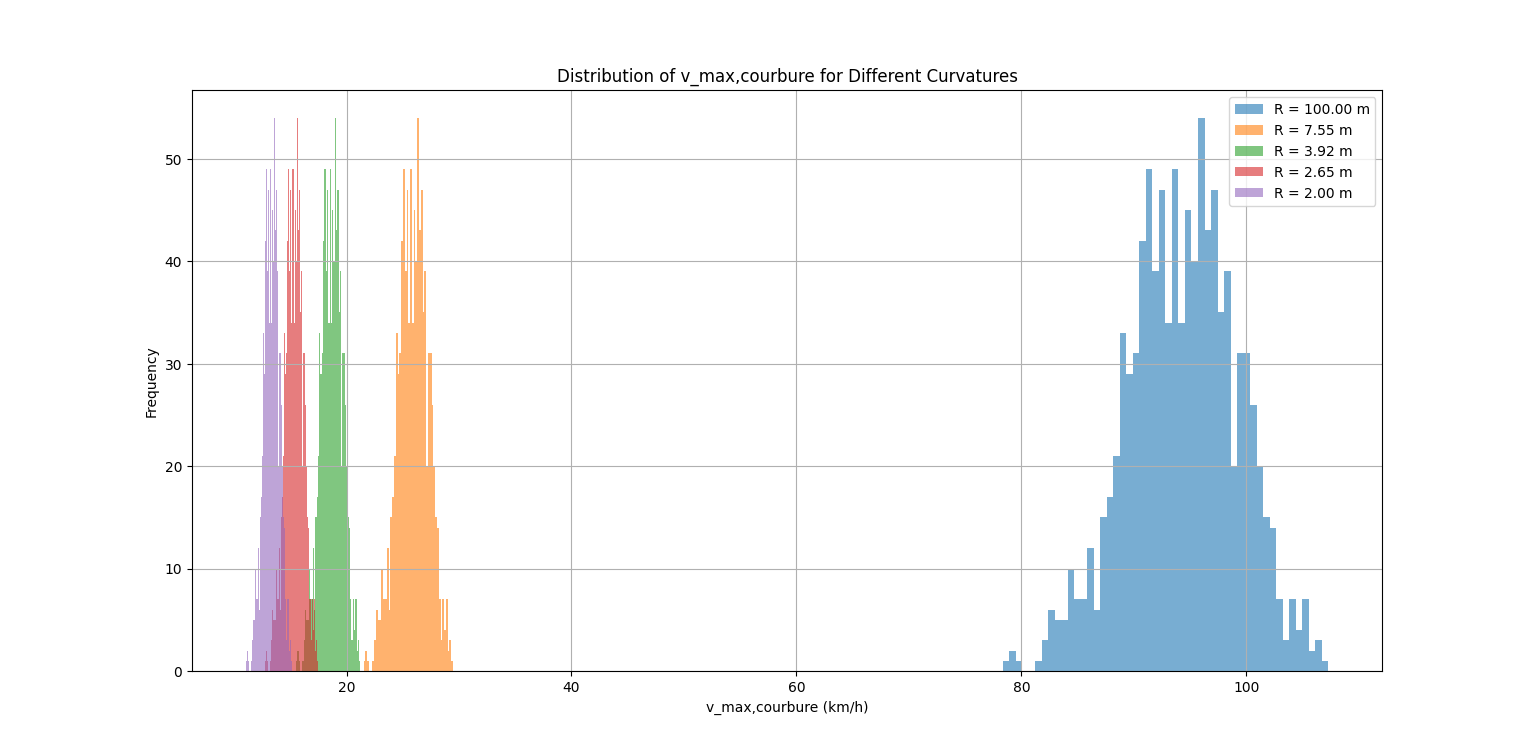
\includegraphics[width=1\linewidth]{Speed vs Curvature.png}

\end{figure}

\section{Introduction de la Variabilité des Conducteurs}

Pour modéliser la variabilité du comportement des conducteurs, nous introduisons une variable aléatoire gaussienne \( X \sim \mathcal{N}(1, \sigma^2) \). Cette variable aléatoire représente la proportion des conducteurs à décélérer différemment dans les virages, ce qui affecte la décélération maximale réelle qu'ils peuvent supporter.

\subsection{Décélération Maximale Réelle}

La décélération maximale réelle que peut supporter un conducteur est influencée par la variable aléatoire \( X \). L'accélération latérale maximale devient donc :

\[
a_{\text{lat}}^{\text{max}} = \mu g X
\]

\subsection{Vitesse Maximale avec Variabilité}

En tenant compte de la variabilité des conducteurs, la vitesse maximale \( v_{\text{max, courbure}} \) dans un virage est modifiée par \( X \) :

\[
v_{\text{max, courbure}} = \sqrt{\frac{\mu g X}{\kappa(s)}} \tag{2-bis}
\]

Cette équation (2-bis) montre que la vitesse maximale dépend non seulement de la courbure de la route, mais aussi de la distribution statistique du comportement des conducteurs.

\subsection{Espérance et Écart-type de la Vitesse Maximale}

Pour une variable \( X \) suivant une distribution normale \( \mathcal{N}(1, \sigma^2) \), l'espérance de la vitesse maximale \( v_{\text{max, courbure}} \) est approximativement :

\[
\mathbb{E}[v_{\text{max, courbure}}] \approx \sqrt{\frac{\mu g}{\kappa(s)}} \sqrt{1 + \frac{\sigma^2}{2}}
\]

L'écart-type de la vitesse maximale \( v_{\text{max, courbure}} \) est approximativement :

\[
\sigma_{v_{\text{max, courbure}}} \approx \sqrt{\frac{\mu g}{\kappa(s)}} \cdot \frac{\sigma}{2}
\]

Ces formules montrent que la variabilité du comportement des conducteurs influence directement la vitesse maximale sécuritaire dans les virages, avec une augmentation de l'écart-type entraînant une plus grande dispersion des vitesses maximales possibles.

\section{Influence de la Pente sur l'Accélération}

Les pentes affectent directement l'accélération des véhicules. Lorsque le véhicule monte ou descend une pente, l'accélération doit être ajustée pour tenir compte de la composante gravitationnelle le long de la pente.

\subsection{Détermination de l'Angle de la Pente}

L'angle \(\theta(s)\) de la pente à la position \(s\) le long de la route peut être déterminé en utilisant le vecteur tangent \(\vec{T}(s)\) et le vecteur de la gravité \(\vec{g}\).

Le vecteur de la gravité \(\vec{g}\) est :

\[
\vec{g} = \begin{pmatrix}
0 \\
0 \\
-g
\end{pmatrix}
\]

L'angle \(\theta(s)\) entre \(\vec{T}(s)\) et \(\vec{g}\) peut être déterminé par le produit scalaire :

\[
\cos(\theta(s)) = \frac{\vec{T}(s) \cdot \vec{g}}{|\vec{T}(s)| |\vec{g}|}
\]

\subsection{Influence sur l'Accélération}

Pour modéliser l'effet de la pente, nous ajustons l'accélération longitudinale en tenant compte de l'angle de la pente \(\theta(s)\). Nous considérons que le conducteur réagit en ajustant son accélération pour compenser la pente.

\paragraph{Accélération Longitudinale Ajustée :}

Lorsque le véhicule monte une pente (\(\theta(s) > 0\)), la composante de la gravité le ralentit, et lorsque le véhicule descend une pente (\(\theta(s) < 0\)), la composante de la gravité l'accélère. Nous modélisons cela par une composante d'accélération supplémentaire :

\[
a_{\text{long, pente}} = a_{\text{long}} - g \sin(\theta(s)) \tag{3}
\]

où :
\begin{itemize}
    \item \(a_{\text{long}}\) est l'accélération longitudinale due au contrôle du véhicule (accélération ou freinage).
    \item \(g \sin(\theta(s))\) est la composante de la gravité le long de la pente.
\end{itemize}

\end{document}
